% !TEX program = xelatex
%
% 分治算法作业
%
\documentclass[12pt,twoside]{article}

% 该模板是《算法设计与分析》课程习题,修改自MIT 6.006
%2021.1.27 增加了中文
\newcommand{\name}{}

\usepackage{amssymb}
\usepackage{amsmath}
\usepackage{graphicx}
\usepackage{latexsym}
\usepackage{times,url}
\usepackage{cprotect}
\usepackage{listings}
\usepackage{graphicx}
\usepackage[table]{xcolor}
\usepackage[letterpaper]{geometry}
\usepackage{enumerate}
\usepackage{forest}
\usepackage{tikz-qtree}
\usepackage{tikz}       % 用于画图的包
\usepackage[linesnumbered,lined,commentsnumbered,ruled]{algorithm2e}  % 用于写伪代码
\usepackage{xeCJK} 			% 写中文要用到
\newcommand{\forcond}{$i=0$ \KwTo $n$} %用于伪代码
\SetKwProg{Fn}{Function}{}{end}
\SetAlgoLongEnd

%===========================段落设置================================================ 
\usepackage{setspace} 
\setlength{\parindent}{2em} 
\setlength{\parskip}{1ex plus 0.5ex minus 0.2ex} 
\linespread{1.35}

\renewcommand\figurename{图} %
\renewcommand\tablename{表}%
%%%%%

\newcommand{\profs}{{\bf 教师}: 杜嘉欣}
\newcommand{\subj}{6.006}
\newcommand{\ttt}[1]{{\tt\small #1}}

\definecolor{dkgreen}{rgb}{0,0.6,0}
\definecolor{dkblue}{rgb}{.2,.2,1}
\definecolor{gray}{rgb}{0.5,0.5,0.5}
\definecolor{mauve}{rgb}{0.58,0,0.82}

\lstset{
  language=Python,
  aboveskip=1pc,
  belowskip=1pc,
  basicstyle={\footnotesize\ttfamily},
  numbers=left,
  showstringspaces=false,
  numberstyle={\tiny\color{gray}\ttfamily},
  keywordstyle={\color{dkblue}\ttfamily},
  commentstyle={\color{dkgreen}\ttfamily},
  stringstyle={\color{mauve}\ttfamily},
}

% \lstset{
%   language=Python,
%   aboveskip=1pc,
%   belowskip=1pc,
%   basicstyle={\bf\color{white}\ttfamily},
%   numbers=left,
%   showstringspaces=false,
%   numberstyle={\bf\small\color{lightgray}\ttfamily},
%   keywordstyle={\bf\color{cyan}\ttfamily},
%   commentstyle={\bf\color{green}\ttfamily},
%   stringstyle={\bf\color{mauve}\ttfamily},
% }


\tikzset{
  % every node/.style={minimum width=2em,draw,circle},
  % level 1/.style={sibling distance=2cm},
  level distance=1cm,
  edge from parent/.style=
  {draw,edge from parent path={(\tikzparentnode) -- (\tikzchildnode)}},
}
\usetikzlibrary{shapes}

\newif\ifHideSolutions
\newcommand{\solution}[1]{\color{dkgreen}\textbf{解答: }#1\color{black}}
\newcommand{\commonmistakes}[1]{{\color{dkblue}\textbf{常见错误: }#1}}
\newcommand{\rubric}[1]{\color{dkgreen}{\bf 说明:} #1\color{black}}

% \HideSolutionsfalse
% \ifHideSolutions
%   \renewcommand{\solution}[1]{}
%   \renewcommand{\rubric}[1]{}
% \fi

\newlength{\toppush}
\setlength{\toppush}{2\headheight}
\addtolength{\toppush}{\headsep}

\newcommand{\htitle}[2]{\noindent\vspace*{-\toppush}\newline\parbox{\textwidth}
{\textit{算法分析与设计}\hfill\name\newline
{\bf 浙江工业大学} \hfill #2\newline
\profs\hfill #1 \\[-3.5ex]\newline
\mbox{}\hrulefill\mbox{}}\vspace*{1ex}\mbox{}\newline
\begin{center}{\Large\bf #1}\end{center}}

\newcommand{\handout}[2]{\thispagestyle{empty}
 \markboth{#1}{#1}
 \pagestyle{myheadings}\htitle{#1}{#2}}

\newcommand{\lecture}[3]{\thispagestyle{empty}
 \markboth{Lecture #1: #2}{Lecture #1: #2}
 \pagestyle{myheadings}\htitle{Lecture #1: #2}{#3}}

\newcommand{\htitlewithouttitle}[2]{\noindent\vspace*{-\toppush}\newline\parbox{6.5in}
{\textit{算法分析与设计}\hfill#2\newline
浙江工业大学 \hfill 6.006\newline
\profs\hfill Handout #1\vspace*{-.5ex}\newline
\mbox{}\hrulefill\mbox{}}\vspace*{1ex}\mbox{}\newline}

\newcommand{\handoutwithouttitle}[2]{\thispagestyle{empty}
 \markboth{Handout \protect\ref{#1}}{Handout \protect\ref{#1}}
 \pagestyle{myheadings}\htitlewithouttitle{\protect\ref{#1}}{#2}}

\newcommand{\exam}[2]{% parameters: exam name, date
 \thispagestyle{empty}
 \markboth{\hspace{1cm}\subj\ #1\hspace{1in}Name\hrulefill\ \ }%
          {\subj\ #1\hspace{1in}Name\hrulefill\ \ }
 \pagestyle{myheadings}\examtitle{#1}{#2}
 \renewcommand{\theproblem}{Problem \arabic{problemnum}}
}
\newcommand{\examsolutions}[3]{% parameters: handout, exam name, date
 \thispagestyle{empty}
 \markboth{Handout \protect\ref{#1}: #2}{Handout \protect\ref{#1}: #2}
% \pagestyle{myheadings}\htitle{\protect\ref{#1}}{#2}{#3}
 \pagestyle{myheadings}\examsolutionstitle{\protect\ref{#1}} {#2}{#3}
 \renewcommand{\theproblem}{Problem \arabic{problemnum}}
}
\newcommand{\examsolutionstitle}[3]{\noindent\vspace*{-\toppush}\newline\parbox{6.5in}
{\textit{Introduction to Algorithms}\hfill#3\newline
Massachusetts Institute of Technology \hfill 6.006\newline
%Singapore-MIT Alliance \hfill SMA5503\newline
\profs\hfill Handout #1\vspace*{-.5ex}\newline
\mbox{}\hrulefill\mbox{}}\vspace*{1ex}\mbox{}\newline
\begin{center}{\Large\bf #2}\end{center}}

\newcommand{\takehomeexam}[2]{% parameters: exam name, date
 \thispagestyle{empty}
 \markboth{\subj\ #1\hfill}{\subj\ #1\hfill}
 \pagestyle{myheadings}\examtitle{#1}{#2}
 \renewcommand{\theproblem}{Problem \arabic{problemnum}}
}

\makeatletter
\newcommand{\exambooklet}[2]{% parameters: exam name, date
 \thispagestyle{empty}
 \markboth{\subj\ #1}{\subj\ #1}
 \pagestyle{myheadings}\examtitle{#1}{#2}
 \renewcommand{\theproblem}{Problem \arabic{problemnum}}
 \renewcommand{\problem}{\newpage
 \item \let\@currentlabel=\theproblem
 \markboth{\subj\ #1, \theproblem}{\subj\ #1, \theproblem}}
}
\makeatother


\newcommand{\examtitle}[2]{\noindent\vspace*{-\toppush}\newline\parbox{6.5in}
{\textit{算法分析与设计}\hfill#2\newline
浙江工业大学 \hfill  2024\newline
%Singapore-MIT Alliance \hfill SMA5503\newline
\profs\hfill #1\vspace*{-.5ex}\newline
\mbox{}\hrulefill\mbox{}}\vspace*{1ex}\mbox{}\newline
\begin{center}{\Large\bf #1}\end{center}}

\newcommand{\grader}[1]{\hspace{1cm}\textsf{\textbf{#1}}\hspace{1cm}}

\newcommand{\points}[1]{[#1 分]\ }
\newcommand{\parts}[1]
{
  \ifnum#1=1
  (1 part)
  \else
  (#1 parts)
  \fi
  \ 
}

\newcommand{\bparts}{\begin{problemparts}}
\newcommand{\eparts}{\end{problemparts}}
\newcommand{\ppart}{\problempart}

%\newcommand{\lg} {lg\ }

\setlength{\oddsidemargin}{0pt}
\setlength{\evensidemargin}{0pt}
\setlength{\textwidth}{6.5in}
\setlength{\topmargin}{0in}
\setlength{\textheight}{8.5in}


\newcommand{\Spawn}{{\bf spawn} }
\newcommand{\Sync}{{\bf sync}}

\renewcommand{\cases}[1]{\left\{ \begin{array}{ll}#1\end{array}\right.}
\newcommand{\cif}[1]{\mbox{if $#1$}}
\newcommand{\cwhen}[1]{\mbox{when $#1$}}

\newcounter{problemnum}
\newcommand{\theproblem}{题目 \theproblemsetnum-\arabic{problemnum}}
\newenvironment{problems}{
        \begin{list}{{\bf \theproblem. \hspace*{0.5em}}}
        {\setlength{\leftmargin}{0em}
         \setlength{\rightmargin}{0em}
         \setlength{\labelwidth}{0em}
         \setlength{\labelsep}{0em}
         \usecounter{problemnum}}}{\end{list}}
\makeatletter
\newcommand{\problem}[1][{}]{\item \let\@currentlabel=\theproblem \textbf{#1}}
\makeatother

\newcounter{problempartnum}[problemnum]
\newenvironment{problemparts}{
        \begin{list}{{\bf (\alph{problempartnum})}}
        {\setlength{\leftmargin}{2.5em}
         \setlength{\rightmargin}{2.5em}
         \setlength{\labelsep}{0.5em}}}{\end{list}}
\newcommand{\problempart}{\addtocounter{problempartnum}{1}\item}

\newenvironment{truefalseproblemparts}{
        \begin{list}{{\bf (\alph{problempartnum})\ \ \ T\ \ F\hfil}}
        {\setlength{\leftmargin}{4.5em}
         \setlength{\rightmargin}{2.5em}
         \setlength{\labelsep}{0.5em}
         \setlength{\labelwidth}{4.5em}}}{\end{list}}

\newcounter{exercisenum}
\newcommand{\theexercise}{Exercise \theproblemsetnum-\arabic{exercisenum}}
\newenvironment{exercises}{
        \begin{list}{{\bf \theexercise. \hspace*{0.5em}}}
        {\setlength{\leftmargin}{0em}
         \setlength{\rightmargin}{0em}
         \setlength{\labelwidth}{0em}
         \setlength{\labelsep}{0em}
        \usecounter{exercisenum}}}{\end{list}}
\makeatletter
\newcommand{\exercise}{\item \let\@currentlabel=\theexercise}
\makeatother

\newcounter{exercisepartnum}[exercisenum]
%\newcommand{\problem}[1]{\medskip\mbox{}\newline\noindent{\bf Problem #1.}\hspace*{1em}}
%\newcommand{\exercise}[1]{\medskip\mbox{}\newline\noindent{\bf Exercise #1.}\hspace*{1em}}

\newenvironment{exerciseparts}{
        \begin{list}{{\bf (\alph{exercisepartnum})}}
        {\setlength{\leftmargin}{2.5em}
         \setlength{\rightmargin}{2.5em}
         \setlength{\labelsep}{0.5em}}}{\end{list}}
\newcommand{\exercisepart}{\addtocounter{exercisepartnum}{1}\item}


% Macros to make captions print with small type and 'Figure xx' in bold.
\makeatletter
\def\fnum@figure{{\bf Figure \thefigure}}
\def\fnum@table{{\bf Table \thetable}}
\let\@mycaption\caption
%\long\def\@mycaption#1[#2]#3{\addcontentsline{\csname
%  ext@#1\endcsname}{#1}{\protect\numberline{\csname 
%  the#1\endcsname}{\ignorespaces #2}}\par
%  \begingroup
%    \@parboxrestore
%    \small
%    \@makecaption{\csname fnum@#1\endcsname}{\ignorespaces #3}\par
%  \endgroup}
%\def\mycaption{\refstepcounter\@captype \@dblarg{\@mycaption\@captype}}
%\makeatother
\let\mycaption\caption
%\newcommand{\figcaption}[1]{\mycaption[]{#1}}

\newcounter{totalcaptions}
\newcounter{totalart}

\newcommand{\figcaption}[1]{\addtocounter{totalcaptions}{1}\caption[]{#1}}

% \psfigures determines what to do for figures:
%       0 means just leave vertical space
%       1 means put a vertical rule and the figure name
%       2 means insert the PostScript version of the figure
%       3 means put the figure name flush left or right
\newcommand{\psfigures}{0}
\newcommand{\spacefigures}{\renewcommand{\psfigures}{0}}
\newcommand{\rulefigures}{\renewcommand{\psfigures}{1}}
\newcommand{\macfigures}{\renewcommand{\psfigures}{2}}
\newcommand{\namefigures}{\renewcommand{\psfigures}{3}}

\newcommand{\figpart}[1]{{\bf (#1)}\nolinebreak[2]\relax}
\newcommand{\figparts}[2]{{\bf (#1)--(#2)}\nolinebreak[2]\relax}


\macfigures     % STATE

% When calling \figspace, make sure to leave a blank line afterward!!
% \widefigspace is for figures that are more than 28pc wide.
\newlength{\halffigspace} \newlength{\wholefigspace}
\newlength{\figruleheight} \newlength{\figgap}
\newcommand{\setfiglengths}{\ifnum\psfigures=1\setlength{\figruleheight}{\hruleheight}\setlength{\figgap}{1em}\else\setlength{\figruleheight}{0pt}\setlength{\figgap}{0em}\fi}
\newcommand{\figspace}[2]{\ifnum\psfigures=0\leavefigspace{#1}\else%
\setfiglengths%
\setlength{\wholefigspace}{#1}\setlength{\halffigspace}{.5\wholefigspace}%
\rule[-\halffigspace]{\figruleheight}{\wholefigspace}\hspace{\figgap}#2\fi}
\newlength{\widefigspacewidth}
% Make \widefigspace put the figure flush right on the text page.
\newcommand{\widefigspace}[2]{
\ifnum\psfigures=0\leavefigspace{#1}\else%
\setfiglengths%
\setlength{\widefigspacewidth}{28pc}%
\addtolength{\widefigspacewidth}{-\figruleheight}%
\setlength{\wholefigspace}{#1}\setlength{\halffigspace}{.5\wholefigspace}%
\makebox[\widefigspacewidth][r]{#2\hspace{\figgap}}\rule[-\halffigspace]{\figruleheight}{\wholefigspace}\fi}
\newcommand{\leavefigspace}[1]{\setlength{\wholefigspace}{#1}\setlength{\halffigspace}{.5\wholefigspace}\rule[-\halffigspace]{0em}{\wholefigspace}}

% Commands for including figures with macpsfig.
% To use these commands, documentstyle ``macpsfig'' must be specified.
\newlength{\macfigfill}
\makeatother
\newlength{\bbx}
\newlength{\bby}
\newcommand{\macfigure}[5]{\addtocounter{totalart}{1}
\ifnum\psfigures=2%
\setlength{\bbx}{#2}\addtolength{\bbx}{#4}%
\setlength{\bby}{#3}\addtolength{\bby}{#5}%
\begin{flushleft}
\ifdim#4>28pc\setlength{\macfigfill}{#4}\addtolength{\macfigfill}{-28pc}\hspace*{-\macfigfill}\fi%
\mbox{\psfig{figure=./#1.ps,%
bbllx=#2,bblly=#3,bburx=\bbx,bbury=\bby}}
\end{flushleft}%
\else\ifdim#4>28pc\widefigspace{#5}{#1}\else\figspace{#5}{#1}\fi\fi}
\makeatletter

\newlength{\savearraycolsep}
\newcommand{\narrowarray}[1]{\setlength{\savearraycolsep}{\arraycolsep}\setlength{\arraycolsep}{#1\arraycolsep}}
\newcommand{\normalarray}{\setlength{\arraycolsep}{\savearraycolsep}}

\newcommand{\hint}{{\bf Hint:\ }}

% Macros from /th/u/clr/mac.tex

\newcommand{\set}[1]{\left\{ #1 \right\}}
\newcommand{\abs}[1]{\left| #1\right|}
\newcommand{\card}[1]{\left| #1\right|}
\newcommand{\floor}[1]{\left\lfloor #1 \right\rfloor}
\newcommand{\ceil}[1]{\left\lceil #1 \right\rceil}
\newcommand{\ang}[1]{\ifmmode{\left\langle #1 \right\rangle}
   \else{$\left\langle${#1}$\right\rangle$}\fi}
        % the \if allows use outside mathmode,
        % but will swallow following space there!
\newcommand{\paren}[1]{\left( #1 \right)}
\newcommand{\bracket}[1]{\left[ #1 \right]}
\newcommand{\prob}[1]{\Pr\left\{ #1 \right\}}
\newcommand{\Var}{\mathop{\rm Var}\nolimits}
\newcommand{\expect}[1]{{\rm E}\left[ #1 \right]}
\newcommand{\expectsq}[1]{{\rm E}^2\left[ #1 \right]}
\newcommand{\variance}[1]{{\rm Var}\left[ #1 \right]}
\renewcommand{\choose}[2]{{{#1}\atopwithdelims(){#2}}}
\def\pmod#1{\allowbreak\mkern12mu({\rm mod}\,\,#1)}
\newcommand{\matx}[2]{\left(\begin{array}{*{#1}{c}}#2\end{array}\right)}
\newcommand{\Adj}{\mathop{\rm Adj}\nolimits}

\newtheorem{theorem}{Theorem}
\newtheorem{lemma}[theorem]{Lemma}
\newtheorem{corollary}[theorem]{Corollary}
\newtheorem{xample}{Example}
\newtheorem{definition}{Definition}
\newenvironment{example}{\begin{xample}\rm}{\end{xample}}
\newcommand{\proof}{\noindent{\em Proof.}\hspace{1em}}
\def\squarebox#1{\hbox to #1{\hfill\vbox to #1{\vfill}}}
\newcommand{\qedbox}{\vbox{\hrule\hbox{\vrule\squarebox{.667em}\vrule}\hrule}}
\newcommand{\qed}{\nopagebreak\mbox{}\hfill\qedbox\smallskip}
\newcommand{\eqnref}[1]{(\protect\ref{#1})}

%%\newcommand{\twodots}{\mathinner{\ldotp\ldotp}}
\newcommand{\transpose}{^{\mbox{\scriptsize \sf T}}}
\newcommand{\amortized}[1]{\widehat{#1}}

\newcommand{\punt}[1]{}

%%% command for putting definitions into boldface
% New style for defined terms, as of 2/23/88, redefined by THC.
\newcommand{\defn}[1]{{\boldmath\textit{\textbf{#1}}}}
\newcommand{\defi}[1]{{\textit{\textbf{#1\/}}}}

\newcommand{\red}{\leq_{\rm P}}
\newcommand{\lang}[1]{%
\ifmmode\mathord{\mathcode`-="702D\rm#1\mathcode`\-="2200}\else{\rm#1}\fi}

%\newcommand{\ckt}[1]{\ifmmode\mathord{\mathcode`-="702D\sc #1\mathcode`\-="2200}\else$\mathord{\mathcode`-="702D\sc #1\mathcode`\-="2200}$\fi}
\newcommand{\ckt}[1]{\ifmmode \sc #1\else$\sc #1$\fi}

%% Margin notes - use \notesfalse to turn off notes.
\setlength{\marginparwidth}{0.6in}
\reversemarginpar
\newif\ifnotes
\notestrue
\newcommand{\longnote}[1]{
  \ifnotes
    {\medskip\noindent Note: \marginpar[\hfill$\Longrightarrow$]
      {$\Longleftarrow$}{#1}\medskip}
  \fi}
\newcommand{\note}[1]{
  \ifnotes
    {\marginpar{\tiny \raggedright{#1}}}
  \fi}


\newcommand{\reals}{\mathbbm{R}}
\newcommand{\integers}{\mathbbm{Z}}
\newcommand{\naturals}{\mathbbm{N}}
\newcommand{\rationals}{\mathbbm{Q}}
\newcommand{\complex}{\mathbbm{C}}

\newcommand{\oldreals}{{\bf R}}
\newcommand{\oldintegers}{{\bf Z}}
\newcommand{\oldnaturals}{{\bf N}}
\newcommand{\oldrationals}{{\bf Q}}
\newcommand{\oldcomplex}{{\bf C}}

\newcommand{\w}{\omega}                 %% for fft chapter

\newenvironment{closeitemize}{\begin{list}
{$\bullet$}
{\setlength{\itemsep}{-0.2\baselineskip}
\setlength{\topsep}{0.2\baselineskip}
\setlength{\parskip}{0pt}}}
{\end{list}}

% These are necessary within a {problems} environment in order to restore
% the default separation between bullets and items.
\newenvironment{normalitemize}{\setlength{\labelsep}{0.5em}\begin{itemize}}
                              {\end{itemize}}
\newenvironment{normalenumerate}{\setlength{\labelsep}{0.5em}\begin{enumerate}}
                                {\end{enumerate}}

%\def\eqref#1{Equation~(\ref{eq:#1})}
%\newcommand{\eqref}[1]{Equation (\ref{eq:#1})}
\newcommand{\eqreftwo}[2]{Equations (\ref{eq:#1}) and~(\ref{eq:#2})}
\newcommand{\ineqref}[1]{Inequality~(\ref{ineq:#1})}
\newcommand{\ineqreftwo}[2]{Inequalities (\ref{ineq:#1}) and~(\ref{ineq:#2})}

\newcommand{\figref}[1]{Figure~\ref{fig:#1}}
\newcommand{\figreftwo}[2]{Figures \ref{fig:#1} and~\ref{fig:#2}}

\newcommand{\liref}[1]{line~\ref{li:#1}}
\newcommand{\Liref}[1]{Line~\ref{li:#1}}
\newcommand{\lirefs}[2]{lines \ref{li:#1}--\ref{li:#2}}
\newcommand{\Lirefs}[2]{Lines \ref{li:#1}--\ref{li:#2}}
\newcommand{\lireftwo}[2]{lines \ref{li:#1} and~\ref{li:#2}}
\newcommand{\lirefthree}[3]{lines \ref{li:#1}, \ref{li:#2}, and~\ref{li:#3}}

\newcommand{\lemlabel}[1]{\label{lem:#1}}
\newcommand{\lemref}[1]{Lemma~\ref{lem:#1}} 

\newcommand{\exref}[1]{Exercise~\ref{ex:#1}}

\newcommand{\handref}[1]{Handout~\ref{#1}}

\newcommand{\defref}[1]{Definition~\ref{def:#1}}

% (1997.8.16: Victor Luchangco)
% Modified \hlabel to only get date and to use handouts counter for number.
%   New \handout and \handoutwithouttitle commands in newmac.tex use this.
%   The date is referenced by <label>-date.
%   (Retained old definition as \hlabelold.)
%   Defined \hforcelabel to use an argument instead of the handouts counter.

\newcounter{handouts}
\setcounter{handouts}{0}

\newcommand{\hlabel}[2]{%
\stepcounter{handouts}
{\edef\next{\write\@auxout{\string\newlabel{#1}{{\arabic{handouts}}{0}}}}\next}
\write\@auxout{\string\newlabel{#1-date}{{#2}{0}}}
}

\newcommand{\hforcelabel}[3]{%          Does not step handouts counter.
\write\@auxout{\string\newlabel{#1}{{#2}{0}}}
\write\@auxout{\string\newlabel{#1-date}{{#3}{0}}}}


% less ugly underscore
% --juang, 2008 oct 05
\renewcommand{\_}{\vrule height 0 pt depth 0.4 pt width 0.5 em \,}

% multiline framed box (will always extend to the far right edge; for a short single line, use \fbox directly)
% --zabel, fall 2018
\newcommand\framepar[1]{\fbox{\begin{minipage}{\linewidth}#1\end{minipage}}}

% 用于显示问题的实例输出
% --Zhenbo Cheng, 2021.02.12
\newenvironment{probexamples}[3]
  {
    \par\noindent\rule{\textwidth}{0.1pt}
      \begin{itemize}
        \setlength\itemsep{0.0em}
        \item[]{\bf 输入: }
        \item[]  #1
        \item[]{\bf 输出: }
        \item[] #2
        \ifx&#3&   \else 
        \item[]{\bf 解释: }
        \item[] #3 \fi 
      \end{itemize}   
  }{}


\newcommand{\theproblemsetnum}{2}
\newcommand{\releasedate}{2025.3.20}
\newcommand{\partaduedate}{ 2025.3.27}

% 必要的包
\usepackage{amsmath}
\usepackage{listings}

%\title{ 习题 3}

\begin{document}

\handout{实验 \theproblemsetnum}{\releasedate}
\textbf{提交截止时间 {\bf \partaduedate}}。本次习题主要涉及分治算法。请用\LaTeX 编辑所有解答。所有问题请给出简洁的回答,任何冗余的回答可能会得低分。

\setlength{\parindent}{0pt}
\medskip\hrulefill\medskip

{\bf 姓名:} xxx\\
{\bf 学号:} xxxxxxxx\\


\medskip

\medskip\hrulefill

\begin{problems}

\problem {\bf 高效求解幂函数}\\
给定两个整数$x$和$n$,其中$n$是非负整数,按照要求计算$x$的$n$次方,也就是$pow(x,n)$。

\bparts
\ppart 给出一个简单遍历的算法求解该问题,要求时间复杂度为$O(n)$。

\textbf{解答}:使用迭代方法计算 $x^n$,通过循环 $n$ 次,每次将结果乘以 $x$。

\begin{lstlisting}[language=C++]
double power(double x, int n) {
    double result = 1;
    for(int i = 1; i <= n; i++) {
        result = result * x;
    }
    return result;
}
\end{lstlisting}

时间复杂度为 $O(n)$,因为需要循环 $n$ 次。

\ppart 给出分治算法求解该问题的步骤,要求时间复杂度为$O(\log n)$。

\textbf{解答}:使用分治策略快速计算幂函数:

\begin{enumerate}
\item 如果 $n = 0$,则返回 1
\item 递归计算 $y = x^{\lfloor n/2 \rfloor}$
\item 如果 $n$ 是偶数,返回 $y^2$
\item 如果 $n$ 是奇数,返回 $y^2 \times x$
\end{enumerate}

该分治算法利用了指数运算的性质:$x^n = x^{n/2} \times x^{n/2}$ (当 $n$ 为偶数) 
或 $x^n = x^{n/2} \times x^{n/2} \times x$ (当 $n$ 为奇数)。

这样每次递归调用将问题规模缩小一半,因此时间复杂度为 $O(\log n)$。

\ppart 给出分治算法求解的代码。

\textbf{解答}:以下是分治算法的 C++ 实现:

\begin{lstlisting}[language=C++]
double power(double x, int n) {
    // 基本情况
    if (n == 0) return 1;
    
    // 处理负指数
    if (n < 0) {
        return 1.0 / power(x, -n);
    }
    
    // 分治部分:计算 x^(n/2)
    double half = power(x, n / 2);
    
    // 根据 n 的奇偶性合并结果
    if (n % 2 == 0) {
        return half * half;
    } else {
        return half * half * x;
    }
}
\end{lstlisting}

\eparts

\newpage
\problem {\bf 字符串最长公共前缀}  \\
给定$n$个字符串,返回这些字符串最长的公共前缀。比如输入字符串序列是 technique, 
technician, technology, technical,那么应该返回techni。
\bparts
\ppart 如果输入字符串序列中,最长的一个字符串长度为$m$,描述一个时间复杂度为$O(mn)$的算法求解该问题。

\textbf{解答}:一个简单的 $O(mn)$ 的算法是:

\begin{enumerate}
\item 取字符串数组中的第一个字符串作为初始的最长公共前缀(LCP)
\item 依次遍历剩余的 $n-1$ 个字符串,对于每个字符串:
   \begin{enumerate}
   \item 从头开始逐字符比较当前字符串与 LCP
   \item 如果发现不匹配,就将 LCP 截断到当前位置
   \item 如果当前字符串比 LCP 短,也要将 LCP 截断到当前字符串的长度
   \end{enumerate}
\end{enumerate}

这个算法需要遍历 $n$ 个字符串,对于每个字符串最多需要比较 $m$ 个字符
(即最长字符串的长度),因此总时间复杂度为 $O(mn)$。

\ppart 描述一个时间复杂度为$O(m\log n)$的算法求解该问题。

\textbf{解答}:使用分治法可以降低时间复杂度:

\begin{enumerate}
\item 将 $n$ 个字符串分成两部分,每部分约有 $n/2$ 个字符串
\item 递归地计算左半部分的最长公共前缀 LCP\_left
\item 递归地计算右半部分的最长公共前缀 LCP\_right
\item 合并两个结果,即找到 LCP\_left 和 LCP\_right 的最长公共前缀
\end{enumerate}

递归的基本情况是当只有一个字符串时,LCP 就是该字符串本身。

在每一层递归中,合并操作的时间复杂度为 $O(m)$,其中 $m$ 是最长字符串的长度。
递归树的高度为 $\log n$,因此总的时间复杂度为 $O(m \log n)$。

\ppart 给出以上时间复杂度为$O(mn)$算法的实现。

\textbf{解答}:以下是 $O(mn)$ 算法的 C++ 实现:

\begin{lstlisting}[language=C++]
#include <iostream>
#include <vector>
#include <string>
using namespace std;

string longestCommonPrefix(vector<string>& strs) {
    // 空数组的情况
    if (strs.empty()) return "";
    
    // 以第一个字符串作为初始 LCP
    string prefix = strs[0];
    
    // 逐个比较剩余的字符串
    for (int i = 1; i < strs.size(); i++) {
        // 当 prefix 变为空或遍历完所有字符串时结束
        if (prefix.empty()) break;
        
        int j = 0;
        // 逐字符比较并更新 prefix
        while (j < prefix.length() && j < strs[i].length() && 
               prefix[j] == strs[i][j]) {
            j++;
        }
        
        // 截断 prefix 到匹配的长度
        prefix = prefix.substr(0, j);
    }
    
    return prefix;
}

// 测试代码
int main() {
    vector<string> example = {"technique", "technician", 
                             "technology", "technical"};
    cout << "最长公共前缀: " << longestCommonPrefix(example) << endl;
    return 0;
}
\end{lstlisting}
\eparts


\newpage
\problem {\bf 有序序列中缺失的最小元素} \\
给定一个序列,其中的元素都是有序的非负整数,要求找出其中缺失的最小的那个元素。

\begin{probexamples}
   {0, 1, 2, 6, 9, 11, 15}
   {3}
   {}
\end{probexamples}

\begin{probexamples}
   {1, 2, 3, 4, 6, 9, 11, 15}
   {0}
   {}
\end{probexamples}

\begin{probexamples}
   {0, 1, 2, 3, 4, 5, 6}
   {7}
   {}
\end{probexamples}

\bparts
\ppart 给出一个时间复杂度为$O(n)$的算法求解该问题。

\textbf{解答}:线性扫描算法可以在 $O(n)$ 时间内解决此问题:

\begin{enumerate}
\item 初始化期望的下一个元素 expected = 0
\item 遍历序列中的每个元素 nums[i]
\item 如果 nums[i] 不等于 expected,则 expected 就是缺失的最小非负整数
\item 否则,更新 expected = nums[i] + 1
\item 如果遍历完整个序列还没有返回结果,则返回 expected
\end{enumerate}

该算法的时间复杂度为 $O(n)$,因为只需要遍历一次数组。

\ppart 给出一个时间复杂度为$O(\log n)$的算法求解该问题。

\textbf{解答}:由于序列是有序的,我们可以使用二分查找的思想来设计 $O(\log n)$ 的算法:

\begin{enumerate}
\item 如果数组第一个元素不是 0,则缺失的最小元素是 0
\item 否则,使用二分查找:
   \begin{enumerate}
   \item 初始化左边界 left = 0,右边界 right = 数组长度 - 1
   \item 当 left < right 时循环:
      \begin{enumerate}
      \item 计算中间位置 mid = left + (right - left) / 2
      \item 如果 nums[mid] == mid(即到目前为止没有缺失的元素),
      则缺失的最小元素在右半部分,left = mid + 1
      \item 否则,缺失的最小元素在左半部分,right = mid
      \end{enumerate}
   \item 当循环结束时,返回 left 作为最小缺失元素的位置
   \end{enumerate}
\end{enumerate}

该算法利用了有序序列的特性,如果没有缺失元素,则序列中的每个元素等于其索引值。
时间复杂度为 $O(\log n)$。

\ppart 给出时间复杂度为$O(\log n)$的算法实现代码。

\textbf{解答}:二分查找算法的 C++ 实现:

\begin{lstlisting}[language=C++]
#include <iostream>
#include <vector>
using namespace std;

int findMissingMinimum(vector<int>& nums) {
    // 检查序列是否为空
    if (nums.empty()) return 0;
    
    // 检查第一个元素是否为0
    if (nums[0] != 0) return 0;
    
    // 检查是否只有一个元素
    if (nums.size() == 1) return 1;
    
    int left = 0;
    int right = nums.size() - 1;
    
    // 如果最后一个元素等于其索引,说明缺失的是下一个数
    if (nums[right] == right) return right + 1;
    
    // 二分查找
    while (left < right) {
        int mid = left + (right - left) / 2;
        
        // 如果中间元素等于其索引,说明缺失元素在右侧
        if (nums[mid] == mid) {
            left = mid + 1;
        } else {
            // 否则缺失元素在左侧
            right = mid;
        }
    }
    
    return left;
}

// 测试代码
int main() {
    vector<int> test1 = {0, 1, 2, 6, 9, 11, 15};
    vector<int> test2 = {1, 2, 3, 4, 6, 9, 11, 15};
    vector<int> test3 = {0, 1, 2, 3, 4, 5, 6};
    
    cout << "Test 1: " << findMissingMinimum(test1) << endl; // 应输出 3
    cout << "Test 2: " << findMissingMinimum(test2) << endl; // 应输出 0
    cout << "Test 3: " << findMissingMinimum(test3) << endl; // 应输出 7
    
    return 0;
}
\end{lstlisting}

\eparts



\newpage
\problem {\bf 铺砖问题} \\
地板长度$n$都是 2 的正整数幂,铺的都是唯一的同一种砖 (如图所示的L字形砖), 
但地板上会有一水泥点已经被覆盖,无需再用铺砖 (图中黑的砖块,这个砖块的位置是随机的)。
如果$n=2$,则存在4个方格,其中,除一个方格外,其余3个方格可被一L型条块覆盖;
当$n=4$时,则存在16个方格,其中,除一个方格外,其余15个方格被5个L型条块覆盖。
输入一个正整数$n$,表示棋盘的大小是$n\times n$的。输出一个被L型条块覆盖的$n\times n$棋盘。
该棋盘除一个方格外,其余各方格都被L型条块覆盖住。
给出问题的分治求解过程、时间复杂度分析和实现代码。
\begin{figure}[h]
   \centering
   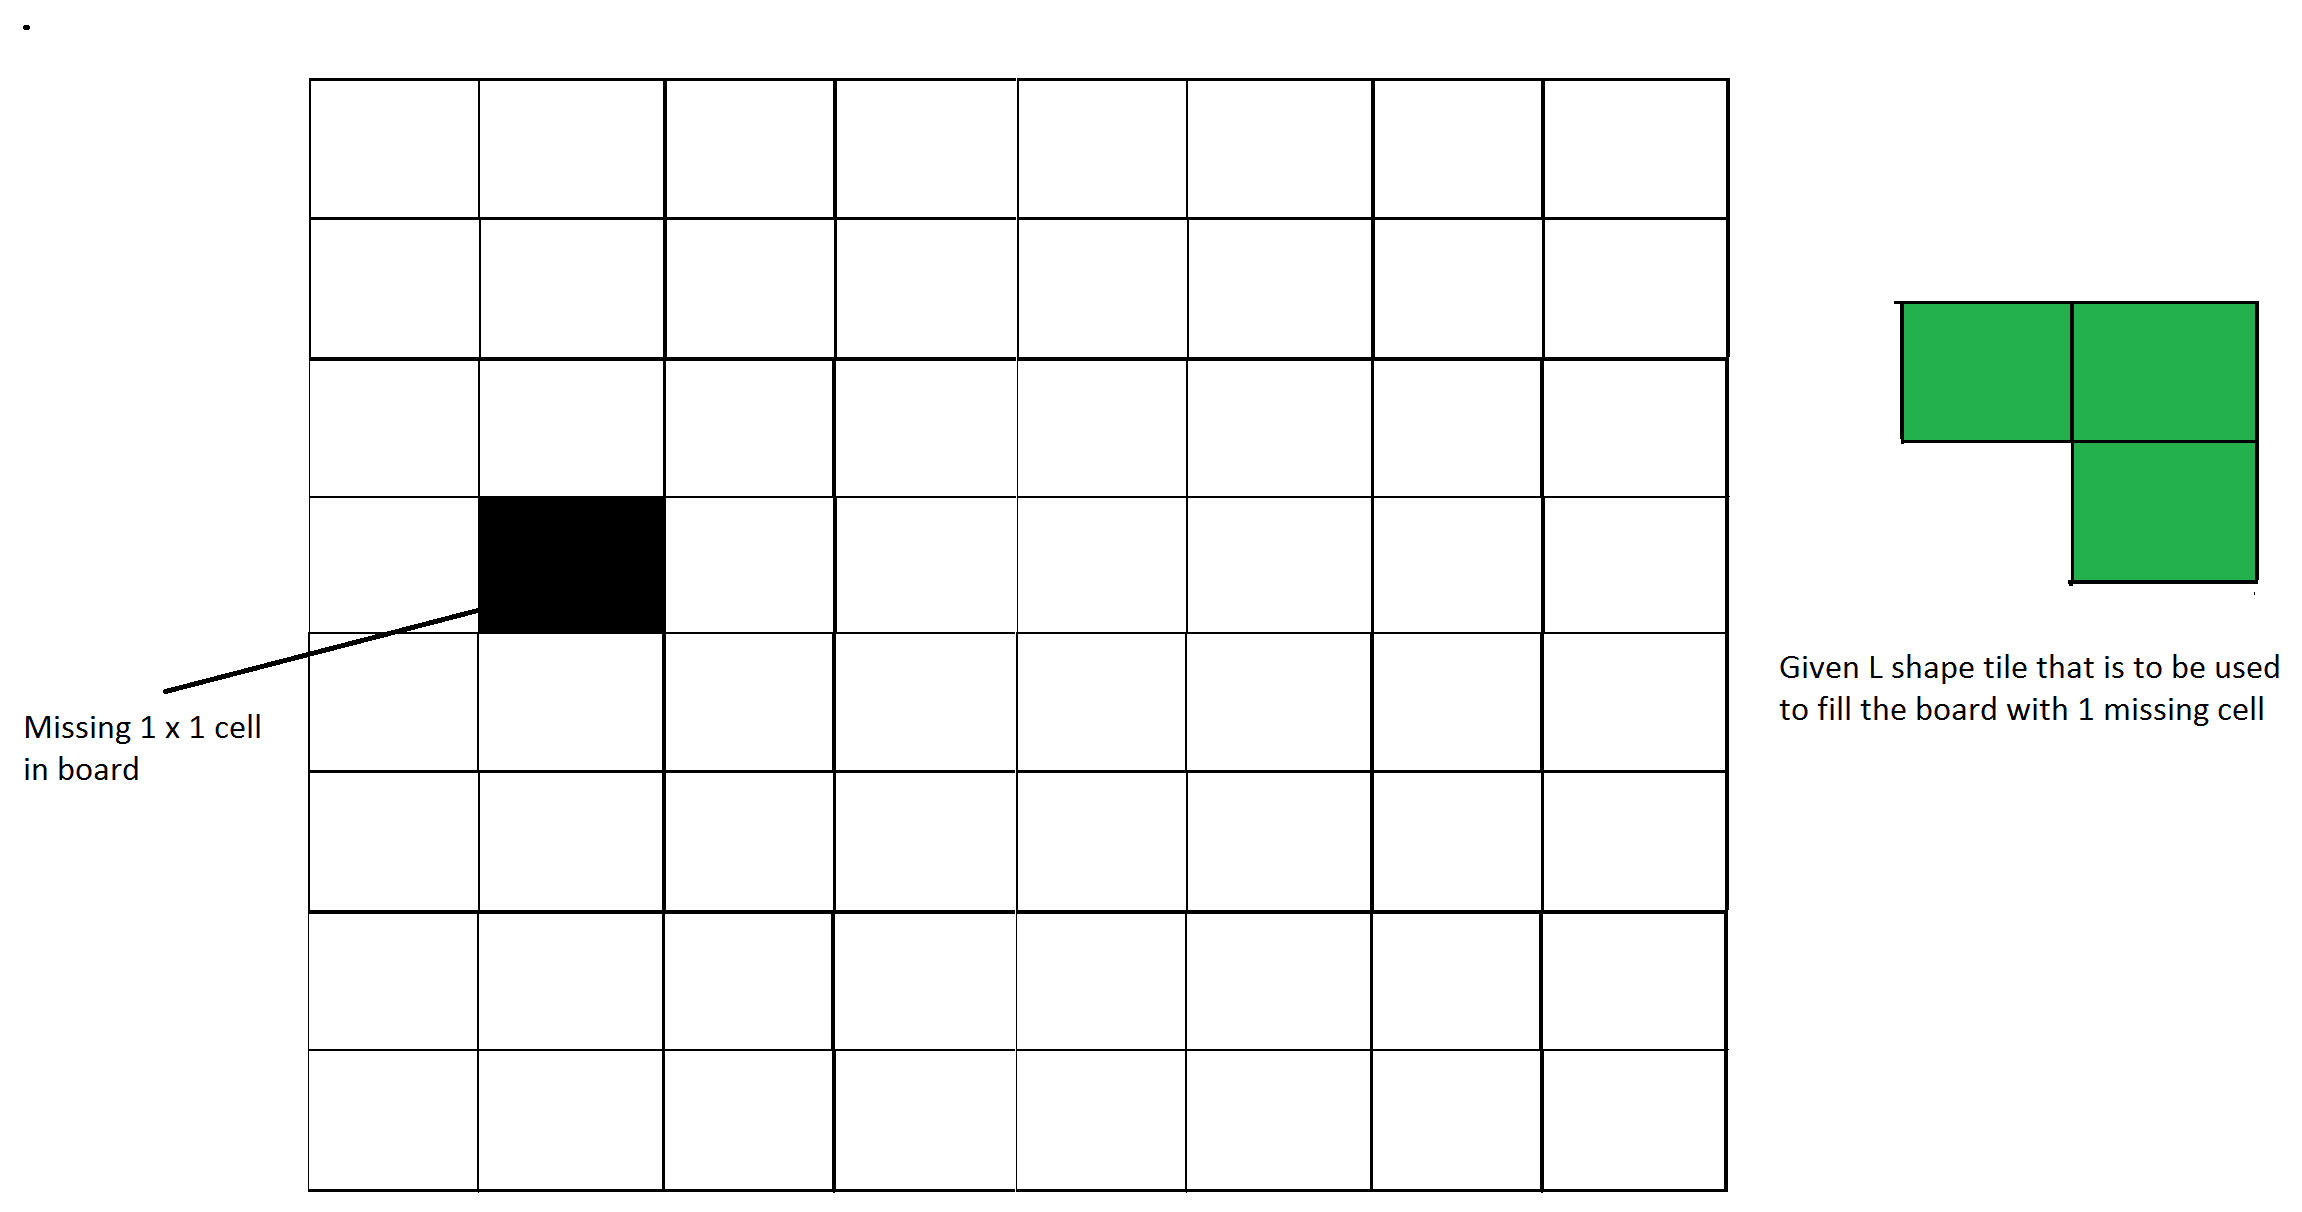
\includegraphics[scale=0.15]{fig/tiles.png}
\end{figure}

\textbf{解答}:

\textbf{分治求解过程}:

\begin{enumerate}
\item \textbf{基本情况}:当 $n=2$ 时,我们有一个 $2 \times 2$ 的棋盘,
其中一个方格已被覆盖,剩余3个方格可以恰好用一个L型砖覆盖。

\item \textbf{分解问题}:对于 $n > 2$ 的情况,我们将 $n \times n$ 的棋盘分成四个 
$n/2 \times n/2$ 的子棋盘。

\item \textbf{确定特殊方格}:在这四个子棋盘中,有一个子棋盘包含原始的特殊方格
(已覆盖的水泥点)。对于其余三个子棋盘,我们需要人为创建一个特殊方格,
使得每个子棋盘都有一个特殊方格。

\item \textbf{放置中心L型砖}:在棋盘的中心放置一个L型砖,使其覆盖四个子棋盘中相邻的三个方格,
这三个方格就是我们在步骤3中创建的特殊方格。

\item \textbf{递归求解}:递归地解决四个 $n/2 \times n/2$ 子棋盘的铺砖问题,
每个子棋盘都有一个特殊方格(一个是原始的,三个是我们创建的)。
\end{enumerate}

\textbf{时间复杂度分析}:

设 $T(n)$ 表示解决大小为 $n \times n$ 的棋盘问题所需的时间。
根据分治算法,我们有:
$T(n) = 4 \times T(n/2) + O(1)$

其中 $O(1)$ 是放置中心L型砖所需的常数时间。

按照主定理,这个递归式的解是 $T(n) = O(n^2)$,因为总共有 $n^2$ 个方格,
我们需要放置 $(n^2-1)/3$ 个L型砖(每个L型砖覆盖3个方格)。

\textbf{代码实现}:

\begin{lstlisting}[language=C++]
#include <iostream>
#include <vector>
#include <cmath>
using namespace std;

// 全局变量,存储棋盘和砖块的编号
vector<vector<int>> board;
int tileNumber = 1;

// 放置L型砖的函数
void placeTile(int row, int col, int specialRow, int specialCol, int size) {
    // 如果只剩下一个2x2的棋盘,直接放置L型砖
    if (size == 2) {
        for (int i = 0; i < 2; i++) {
            for (int j = 0; j < 2; j++) {
                if (row + i != specialRow || col + j != specialCol) {
                    board[row + i][col + j] = tileNumber;
                }
            }
        }
        tileNumber++;
        return;
    }
    
    int halfSize = size / 2;
    int centerRow = row + halfSize - 1;
    int centerCol = col + halfSize - 1;
    
    // 确定特殊方格在哪个象限
    int quadrant;
    if (specialRow <= centerRow && specialCol <= centerCol) {
        quadrant = 0; // 左上角
    } else if (specialRow <= centerRow && specialCol > centerCol) {
        quadrant = 1; // 右上角
    } else if (specialRow > centerRow && specialCol <= centerCol) {
        quadrant = 2; // 左下角
    } else {
        quadrant = 3; // 右下角
    }
    
    // 放置中心L型砖
    int currentTile = tileNumber++;
    
    // 右上角
    if (quadrant != 1) board[centerRow][centerCol + 1] = currentTile;
    // 左下角
    if (quadrant != 2) board[centerRow + 1][centerCol] = currentTile;
    // 右下角
    if (quadrant != 3) board[centerRow + 1][centerCol + 1] = currentTile;
    // 左上角
    if (quadrant != 0) board[centerRow][centerCol] = currentTile;
    
    // 递归处理四个子棋盘
    
    // 左上角子棋盘
    int nextSpecialRow = (quadrant == 0) ? specialRow : centerRow;
    int nextSpecialCol = (quadrant == 0) ? specialCol : centerCol;
    placeTile(row, col, nextSpecialRow, nextSpecialCol, halfSize);
    
    // 右上角子棋盘
    nextSpecialRow = (quadrant == 1) ? specialRow : centerRow;
    nextSpecialCol = (quadrant == 1) ? specialCol : centerCol + 1;
    placeTile(row, col + halfSize, nextSpecialRow, nextSpecialCol, halfSize);
    
    // 左下角子棋盘
    nextSpecialRow = (quadrant == 2) ? specialRow : centerRow + 1;
    nextSpecialCol = (quadrant == 2) ? specialCol : centerCol;
    placeTile(row + halfSize, col, nextSpecialRow, nextSpecialCol, halfSize);
    
    // 右下角子棋盘
    nextSpecialRow = (quadrant == 3) ? specialRow : centerRow + 1;
    nextSpecialCol = (quadrant == 3) ? specialCol : centerCol + 1;
    placeTile(row + halfSize, col + halfSize, 
              nextSpecialRow, nextSpecialCol, halfSize);
}

// 打印棋盘的函数
void printBoard(int n) {
    for (int i = 0; i < n; i++) {
        for (int j = 0; j < n; j++) {
            if (board[i][j] == -1) {
                cout << "S\t"; // 特殊方格
            } else {
                cout << board[i][j] << "\t";
            }
        }
        cout << endl;
    }
}

int main() {
    int n;
    cout << "输入棋盘大小(必须是2的幂): ";
    cin >> n;
    
    // 初始化棋盘
    board.resize(n, vector<int>(n, 0));
    
    // 设置特殊方格的位置(这里设为左上角,可以根据需要修改)
    int specialRow = 0, specialCol = 0;
    cout << "输入特殊方格的位置(行 列): ";
    cin >> specialRow >> specialCol;
    
    // 标记特殊方格
    board[specialRow][specialCol] = -1;
    
    // 解决铺砖问题
    placeTile(0, 0, specialRow, specialCol, n);
    
    // 打印结果
    printBoard(n);
    
    return 0;
}
\end{lstlisting}

\newpage
\problem{\bf 序列逆序对数} \\
给定一个序列$A$,找出序列中逆序对的个数。逆序是当$i<j$和$A[i]>A[j]$同时成立,
那么$A[i]$与$A[j]$构成逆序对。比如$A=[1, 9, 6, 4, 5]$,该序列逆序对数为5,
分别为$[9, 6], [9, 4], [9, 5], [6, 4], [6, 5]$。
\bparts
\ppart 给出一个时间复杂度为$O(n^2)$的算法求解该问题。

\textbf{解答}:一个简单的 $O(n^2)$ 算法是使用双重循环直接枚举所有可能的逆序对:

\begin{enumerate}
\item 初始化逆序对计数器 count = 0
\item 对于每个位置 i(从0到n-2):
   \begin{enumerate}
   \item 对于每个位置 j(从i+1到n-1):
      \begin{enumerate}
      \item 如果 A[i] > A[j],则增加计数器 count++
      \end{enumerate}
   \end{enumerate}
\item 返回最终的计数值 count
\end{enumerate}

这个算法的时间复杂度是 $O(n^2)$,因为我们需要检查 $\binom{n}{2} = \frac{n(n-1)}{2}$ 
个可能的对。

\ppart 给出一个时间复杂度为$O(n\log n)$的算法求解该问题。

\textbf{解答}:使用归并排序的变体可以在 $O(n\log n)$ 时间内计算逆序对:

\begin{enumerate}
\item 实现一个修改版的归并排序,在合并两个已排序子数组时计算逆序对
\item 在归并排序过程中,当右子数组的元素被选择时,不会产生新的逆序对
\item 当左子数组的元素被选择时,右子数组中已经处理的所有元素都与当前左子数组元素构成逆序对
\end{enumerate}

具体步骤如下:
\begin{enumerate}
\item 将数组分成两半
\item 递归统计左半部分的逆序对数量
\item 递归统计右半部分的逆序对数量
\item 在归并两个已排序数组的过程中,统计跨越左右两半部分的逆序对数量
\item 返回总的逆序对数量
\end{enumerate}

由于归并排序的时间复杂度是 $O(n\log n)$,这个算法的总时间复杂度也是 $O(n\log n)$。

\ppart 给出一个时间复杂度为$O(n\log n)$算法的实现代码。

\textbf{解答}:基于归并排序的逆序对计数算法的 C++ 实现:

\begin{lstlisting}[language=C++]
#include <iostream>
#include <vector>
using namespace std;

// 合并两个已排序的子数组并计算逆序对
long long merge(vector<int>& nums, vector<int>& temp, 
                int left, int mid, int right) {
    // i指向左子数组,j指向右子数组
    int i = left;
    int j = mid + 1;
    int k = left; // 指向临时数组的位置
    long long invCount = 0;
    
    while (i <= mid && j <= right) {
        if (nums[i] <= nums[j]) {
            // 左子数组元素小于等于右子数组元素,不构成逆序对
            temp[k++] = nums[i++];
        } else {
            // 左子数组元素大于右子数组元素,构成逆序对
            // 当前左子数组的元素及其后面的所有元素都与当前右子数组元素构成逆序对
            temp[k++] = nums[j++];
            invCount += (mid - i + 1);
        }
    }
    
    // 将剩余元素复制到临时数组
    while (i <= mid) {
        temp[k++] = nums[i++];
    }
    
    while (j <= right) {
        temp[k++] = nums[j++];
    }
    
    // 将临时数组中的元素复制回原数组
    for (i = left; i <= right; i++) {
        nums[i] = temp[i];
    }
    
    return invCount;
}

// 归并排序并计算逆序对
long long mergeSort(vector<int>& nums, vector<int>& temp, 
                    int left, int right) {
    long long invCount = 0;
    
    if (left < right) {
        int mid = left + (right - left) / 2;
        
        // 计算左子数组中的逆序对
        invCount += mergeSort(nums, temp, left, mid);
        
        // 计算右子数组中的逆序对
        invCount += mergeSort(nums, temp, mid + 1, right);
        
        // 计算跨越左右子数组的逆序对
        invCount += merge(nums, temp, left, mid, right);
    }
    
    return invCount;
}

// 计算逆序对数量的主函数
long long countInversions(vector<int>& nums) {
    int n = nums.size();
    vector<int> temp(n);
    return mergeSort(nums, temp, 0, n - 1);
}

int main() {
    vector<int> nums = {1, 9, 6, 4, 5};
    
    cout << "序列: ";
    for (int num : nums) {
        cout << num << " ";
    }
    cout << endl;
    
    long long inversions = countInversions(nums);
    cout << "逆序对数量: " << inversions << endl;
    
    return 0;
}
\end{lstlisting}


\eparts
\end{problems}
\end{document}

